\documentclass[]{article}
\usepackage{lmodern}
\usepackage{amssymb,amsmath}
\usepackage{ifxetex,ifluatex}
\usepackage{fixltx2e} % provides \textsubscript
\ifnum 0\ifxetex 1\fi\ifluatex 1\fi=0 % if pdftex
  \usepackage[T1]{fontenc}
  \usepackage[utf8]{inputenc}
\else % if luatex or xelatex
  \ifxetex
    \usepackage{mathspec}
  \else
    \usepackage{fontspec}
  \fi
  \defaultfontfeatures{Ligatures=TeX,Scale=MatchLowercase}
\fi
% use upquote if available, for straight quotes in verbatim environments
\IfFileExists{upquote.sty}{\usepackage{upquote}}{}
% use microtype if available
\IfFileExists{microtype.sty}{%
\usepackage{microtype}
\UseMicrotypeSet[protrusion]{basicmath} % disable protrusion for tt fonts
}{}
\usepackage[margin=1in]{geometry}
\usepackage{hyperref}
\hypersetup{unicode=true,
            pdftitle={The dating of the Human-Neandertal introgression event estimated from present-day human genomes is compatible with a multitude of admixture durations},
            pdfauthor={Leonardo Nicola Martin Iasi (Max Planck Institute for Evolutionary Anthropology, MPI EVA), Dr.~Benjamin Marco Peter (MPI EVA, benjamin\_peter@eva.mpg.de)},
            pdfborder={0 0 0},
            breaklinks=true}
\urlstyle{same}  % don't use monospace font for urls
\usepackage{natbib}
\bibliographystyle{plainnat}
\usepackage{graphicx,grffile}
\makeatletter
\def\maxwidth{\ifdim\Gin@nat@width>\linewidth\linewidth\else\Gin@nat@width\fi}
\def\maxheight{\ifdim\Gin@nat@height>\textheight\textheight\else\Gin@nat@height\fi}
\makeatother
% Scale images if necessary, so that they will not overflow the page
% margins by default, and it is still possible to overwrite the defaults
% using explicit options in \includegraphics[width, height, ...]{}
\setkeys{Gin}{width=\maxwidth,height=\maxheight,keepaspectratio}
\IfFileExists{parskip.sty}{%
\usepackage{parskip}
}{% else
\setlength{\parindent}{0pt}
\setlength{\parskip}{6pt plus 2pt minus 1pt}
}
\setlength{\emergencystretch}{3em}  % prevent overfull lines
\providecommand{\tightlist}{%
  \setlength{\itemsep}{0pt}\setlength{\parskip}{0pt}}
\setcounter{secnumdepth}{0}
% Redefines (sub)paragraphs to behave more like sections
\ifx\paragraph\undefined\else
\let\oldparagraph\paragraph
\renewcommand{\paragraph}[1]{\oldparagraph{#1}\mbox{}}
\fi
\ifx\subparagraph\undefined\else
\let\oldsubparagraph\subparagraph
\renewcommand{\subparagraph}[1]{\oldsubparagraph{#1}\mbox{}}
\fi

%%% Use protect on footnotes to avoid problems with footnotes in titles
\let\rmarkdownfootnote\footnote%
\def\footnote{\protect\rmarkdownfootnote}

%%% Change title format to be more compact
\usepackage{titling}

% Create subtitle command for use in maketitle
\providecommand{\subtitle}[1]{
  \posttitle{
    \begin{center}\large#1\end{center}
    }
}

\setlength{\droptitle}{-2em}

  \title{The dating of the Human-Neandertal introgression event estimated from present-day human genomes is compatible with a multitude of admixture durations}
    \pretitle{\vspace{\droptitle}\centering\huge}
  \posttitle{\par}
    \author{Leonardo Nicola Martin Iasi (Max Planck Institute for Evolutionary
Anthropology, MPI EVA), Dr.~Benjamin Marco Peter (MPI EVA,
\href{mailto:benjamin_peter@eva.mpg.de}{\nolinkurl{benjamin\_peter@eva.mpg.de}})}
    \preauthor{\centering\large\emph}
  \postauthor{\par}
      \predate{\centering\large\emph}
  \postdate{\par}
    \date{2020-03-24}

\usepackage{setspace}
\doublespacing
\usepackage[none]{hyphenat}
\usepackage{amsfonts}
\usepackage{amssymb}
\usepackage{graphicx}
\usepackage{float}
\usepackage{xcolor}
\floatplacement{figure}{H}

\begin{document}
\maketitle

\section{Abstract}\label{abstract}

\section{Introduction}\label{introduction}

Admixture, i.e. gene flow between populations, is a major evolutionary force that shapes genetic diversity and allows the exchange of beneficial variants. Genomic studies have shown that admixture is prevalent across species (\cite{Salazar_Hybrid_speciation_2010, rieseberg_hybridization_2007,kronforst_multilocus_2006,kolbe_multiple_2007}) and facilitates adaptation (\cite{harrison_hybridization_2014,hedrick_adaptive_2013, shaw_genes_2011,payseur_using_2010}).

The advent of wide-spread full-genome sequencing methods makes it easier to detect admixture events
between populations (\cite{sousa_understanding_2013}). In humans, the sequencing of
the Neandertal genome (\cite{green_draft_2010}) revealed that all humans outside Africa carry low proportions of Neandertal ancestry
(\cite{green_draft_2010,prufer_complete_2013,vernot_resurrecting_2014,fu_early_2015,fu_genome_2014,sankararaman_genomic_2014,prufer_high-coverage_2017}). In addition, the  Denisovan genome (\cite{reich_genetic_2010})
showed low proportions of Denisovan ancestry being widespread in Oceania and to a smaller extent in East-Asia
(\cite{reich_genetic_2010,meyer_high-coverage_2012,sankararaman_combined_2016,vernot_excavating_2016,malaspinas_genomic_2016}).
This genetic evidence for the direct contact and interbreeding of modern humans with other hominin populations can also help resolving the timing and duration of contact by genetically dating the admixture.
Moreover, additional to archaeological records of Neandertals, the admixture can hint to the time of their disappearance assumed to be at the end of the Mousterian around 41,030–39,260 calibrated years before present (yBP) (\cite{higham_timing_2014}), based on archaeological data. 
Together, genetically dated admixture events can be a clue of the debated question of contact with and extinction of these hominin populations.

\subsection{Admixture on the genomic level and basic idea how to date
it}\label{admixture-on-the-genomic-level-and-basic-idea-how-to-date-it}

On the genomic level, admixture introduces  divergent chromosomes
into the admixed population. Over time, meiotic recombination
progressively breaks these chromosomes down into introgressed segments, whose size decreases with time (\cite{falush_inference_2003}). 
Assuming that recombination events are
independent from each other, the length of these segments  is roughly inversely proportional to  the number of
generations since admixture
(\cite{moorjani_history_2011,pool_inference_2009,gravel_population_2012,liang_lengths_2014}).
Hence, using this 'recombination clock', the length distribution of introgressed chromosomal segments
 can be used to inferred the time since the
admixture event 
(\cite{moorjani_history_2011,pugach_dating_2011,sankararaman_date_2012,loh_inferring_2013,sankararaman_combined_2016,pugach_gateway_2018,jacobs_multiple_2019,hellenthal_genetic_2014}).


\subsection{The two approaches and their application to find archaic admixture dates}\label{the-two-approaches-and-their-application-to-find-archaic-admixture-dates}

The first step in dating admixture events from genetic data is estimating the length distribution of admixture segments.  There are two main approaches for this; a first approach is to use patterns of linkage along a chromosome to estimate the length distribution, without explicitly inferring the genomic location of these segments. In contrast, a second set of methods first aims to identify all admixture segments over a certain length, and then use these segments for inference. 
(\cite{chimusa_dating_2018}) (Figure \ref{fig:fig1} A).

The first approach uses the admixture-induced linkage disequilibrium
(ALD) decay. Variants on introgressed archaic segments are
expected to be in high linkage disequilibrium to each other at the time
of admixture
(\cite{chakraborty_admixture_1988,stephens_mapping_1994,wall_detecting_2000}). The extent of linkage between introgressed variants decreases over generations as genetic distance increases. Hence, in case of a recent
admixture event a few tens of generations ago, ALD stretches  over long genetic distances
(\cite{patterson_methods_2004}) and is therefore easily distinguishable
from short range LD due to other processes (\cite{moorjani_history_2011}). For ancient
admixture events however, ALD is quite similar to the genomic background. To circumvent this issue for dating the Neandertal-human admixture time, an ascertainment scheme was used to calculate LD only for markers that are nearly differentially fixed between the two taxa. In this case, the presence of apparent Neandertal alleles in close-range LD is a signature of a locally introgressed locus
(\cite{sankararaman_date_2012}). Typically, estimation of admixture time proceeds by fitting a decay curve of pairwise LD as a function of
genetic distance, using an exponential distribution whose parameters are informative for the time of an admixture pulse
(\cite{moorjani_history_2011,loh_inferring_2013}). Using this approach Sankararaman et al. dated the Neandertal-human admixture time to
be  between 37,000--86,000 ya (years ago) (\cite{sankararaman_date_2012}). Later,
this date was refined to 40,510--54,454 ya (95\% CI) using a different
ascertainment scheme combined with a different genetic map
(\cite{moorjani_genetic_2016}). A date was also obtained from an ancient
genome to be 50,000 - 60,000 ya by adding the time since the admixture obtained from the
ancient individual, by the decay of pairwise covariance between
introgressed SNPs, to the specimens radiocarbon date
(\cite{fu_genome_2014}).

A higher amount of Neandertal admixture segments in present-day East-Asians was identified by using the second set of approaches. To explain the higher amount of Neandertal ancestry in these populations a second admixture event was suggested at the same time as the admixture between Neandertals and
all non-Africans (\cite{kim_selection_2015,vernot_complex_2015}).  The identification of segments is largely independent from the later dating, and can be done using a variety of methods.(\cite{racimo_signatures_2017,seguin_orlando_paleogenomics_2014,vernot_excavating_2016,sankararaman_combined_2016,skov_detecting_2018}. The length distribution of the obtained fragments is then used to estimate the time of the admixture pulse, typically using an exponential model.

The Denisovan human
admixture time point was dated to lie in the interval between 44,000--54,000 ya using the ALD
approach on modern day genomes (\cite{sankararaman_combined_2016}).

Direct identification of archaic segments in genomes from present day Southeast-Asians revealed a proportion of previously unknown Denisovan ancestry private to these populations. The segments from this ancestry are more diverged from the high-coverage Denisovan genome then previously found ones. This suggests an additional admixture event from a different population of Denisovans (\cite{browning_analysis_2018}).
Comparing the mean length of the formerly known and newly identified Denisovan segments did, however, not reveal
significant differences, suggesting a lack of power to distinguish the
two events by time (\cite{browning_analysis_2018,jacobs_multiple_2019}).
Analysing genomes from Papuan individuals revealed two time separated
admixture events with Denisovans, one in line with previous estimates at
45.7 kya (95\% CI 31.9-60.7 kya) and one exclusive to Papuans dated to
be around 29.8 kya (95\% CI 14.4-50.4 kya)
(\cite{jacobs_multiple_2019}).

Here, we are manly interested in the gene flow model these studies used and its implication.

The most widely used model is one where gene flow is constant through time (\cite{nielsen_distinguishing_2001,hey_multilocus_2004}), which does not have a time component. However, for dating admixture, it is generally assumed that gene flow
happens over a very short time period, in a single \textit{admixture pulse} (\cite{moorjani_history_2011}), usually modelled as a single generation
of gene flow. While convenient for inference, one cannot use this approach to distinguish an extend period of gene flow from an admixture pulse (\cite{pickrell_toward_2014}). 
Here, we are chiefly interested in gene flow between Neandertals and modern humans, which was previously modeled assuming a one-generation pulse of admixture. Dating this gene flow event accurately would inform several questions of  great importance, but not always the same aspect of the gene flow is the one of primary interest. For example, if we are interested in dating the out-of-Africa migration of our ancestors, the start of the gene flow between Neandertals and modern humans is of primary interest, as this establishes modern humans and Neandertals in sympatry, likely outside of Africa.
In contrast, the date of the most recent gene flow between Neandertals and modern humans may be informative for dating the extinction of Neandertals. Under an admixture pulse model, which assumes that these two times coincide, hypotheses about the impact of modern human colonization of Eurasia on Neandertal extinction cannot be evaluated.

Thus, our goal here is to examine when an admixture pulse can be rejected for more general models of continuous gene flow (Figure \ref{fig:fig1}.  Using a continuous model, we are interested in establishing the start and end of admixture between Neandertals and modern humans, not just the mean admixture time. This is a difficult problem, as it requires deconvoluting an exponential mixture, which is notoriously hard (\cite{dasgupta_mixture_2008}). Thus, we also need to carefully evaluate the potential technical and biological factors that may introduce additional biases (\cite{pool_inference_2009,gravel_population_2012,liang_lengths_2014}).
For this purpose, we explore these factors influencing the inferred time of admixture pulses, to gauge their relative importance.



\subsection{Assumptions on the data}\label{assumptions-on-the-data}

In general the model assumes that introgressed segments are rare and inbreeding is not significant (\cite{pool_inference_2009}). The segments act neutral (\cite{shchur_distribution_2019}) and the recombination clock is constant over time and populations (\cite{gravel_population_2012}). We will adopt these assumptions. Instead we focus on the one-generation pulse and technical assumptions. It is usually assumed that the demography is known or its effects negligible, the recombination map known or recombination is constant. Beside that it is assumed that the ascertainment scheme sufficiently represent the variation in the true introgressing archaic population.

Violations of these assumptions are known to influence the mean time
estimates. Hence, the effect of assuming a one-generation pulse has to
be contrasted with other influencing factors, for both a scenario of
pulse-like and multi-generation long admixture. 


\subsection{complex migration models}

To relax the one-generation pulse assumption we have to generalize the admixture model.
The simplest generalization of the admixture pulse model to more complex scenarios is to assume a model with two or more pulses. In such a case,  each segment will have entered in one of the pulses, and the resulting admixture tracts will be a discrete mixture of the constituent distributions (\cite{pickrell_ancient_2014}), weighted by the relative migration rates. Zhou et al. 2017 (\cite{zhou_modeling_2017}) showed that this model, in principle, can be used for continuous mixtures as well, using a polynomial function as a mixture density. However, they found that even for relatively short admixture events, the large number of parameters led to an underestimate of admixture duration (\cite{zhou_inference_2017}), and the beginning and end of admixture were not well inferred
(\cite{zhou_modeling_2017,zhou_inference_2017}). 

Here we use a simpler model of continuous admixture with just two parameters, and one less than the two-pulse model of Pickrell et al. 2014 (\cite{pickrell_ancient_2014}). One parameter reflects the mean admixture time, and the other the duration of the admixture event; letting this parameter go to zero thus recovers the (nested) pulse model. 
This model is particularly simple if we assume that migration rate over time is Gamma distributed, in which case the distribution of admixture segment lengths has a closed form (Figure \ref{fig:fig1} B & C).

\subsection{What we want to do}\label{what-we-want-to-do}
In our  study, we first examine the  effect of long
continuous admixture on the admixture time estimates (assuming a pulse-like admixture) in comparison to
the effects of the aforementioned model assumptions. Second, we define
the expectation of the resulting segment length distribution for
continuous Gamma distributed admixture being Lomax distributed, holding
a parameter for the duration of admixture. This expectation works for
both methods to infer the segments length, either directly or by using
the ALD decay. Using this model, we investigate under which scenarios
the parameters of the Lomax-distribution can be accurately estimated and
for which parameters we can distinguish a pulse-like admixture event
from a continuous event. We show that in many cases pulses cannot be
distinguished from more continuous admixture events. Using the 1000 Genomes data, ALD inferred admixture times from Europeans are consistent with a multitude of duration times.
We conclude that current
methods are unsuitable to definitively answer when the contact between
Neandertals and modern humans ended.

\begin{figure}
\centering
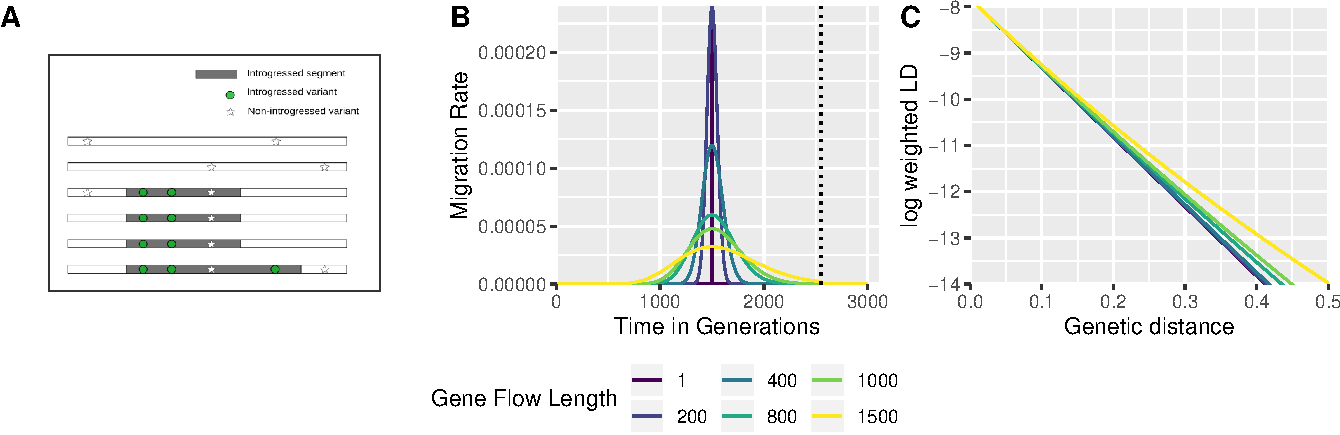
\includegraphics{Admixture_Time_Inference_Paper_Draft_files/figure-latex/fig1-1.pdf}
\caption{\label{fig:fig1} A) Neandertal introgression into non-Africans with a multitude of potential admixture durations. The time and duration of admixture results in different length distributions of introgressed chromosomal segments (grey) containing  Neandertal variants (green circles)  in high LD to each other
compared to the background . The ALD approach estimates linkage
between the introgressed variants (green circles), wheres the haplotype approach tries
to estimate the segment directly (grey area). B) Migration rate per generation
modeled using a Gamma distribution for different admixture durations,
dotted line indicates maximum time of gene flow. C) The expected LD
decay modeled as a Lomax distribution for the different length.}
\end{figure}

\section{Methods}\label{methods}

We conducted various simulations to assess the effect of continuous
admixture compared to a pulse under ideal circumstances. We changed
recombination and demographic parameters to simulate more realistic
models. We compared the effect of these parameters together with
analysis parameters to the effect of continuous admixture on the
estimates. After assessing these effects we evaluate the possible
parameter range for using a Lomax distribution to fit the ALD decay,
enabling to obtain a duration of continuous admixture. To demonstrate our finding we used the 1000 Genomes data together with 3 high coverage Neandertals to fit several gene flow models with different durations to the data.

\subsection{Simulations}\label{simulations}

We used the msprime coalescent simulator
(\cite{kelleher_efficient_2016}) for simulations with sample sizes
chosen to reflect presently available data: We simulate 176 diploid
African individuals and 170 diploid non-Africans, corresponding to the
number of Yoruba (YRI) and Central Europeans from Utah (CEU)
sequences in the 1000 Genomes project data
(\cite{the_1000_genomes_project_consortium_global_2015}). Since three
high coverage Neandertal sequences are available
(\cite{prufer_complete_2013,prufer_high-coverage_2017,mafessoni_high_coverage_2020}) we choose to
simulate three diploid genomes. For each individual we simulated 20
chromosomes with a length of 150 Mb each. The mutation rate was set for
all simulations to \(2*10^{-8}\) per base per generation. The
recombination rate was set to \(1*10^{-8}\) per base pair per generation
unless specified otherwise. The demographic parameters are based on
previous studies dating Neandertal admixture
(\cite{sankararaman_date_2012,fu_genome_2014,moorjani_genetic_2016}). In
the ``simple'' model (Figure \ref{fig:figS1}, the effective
population size is assumed constant at Ne=10000 for all populations, the
split time between modern humans and Neandertals is 10000 generations
ago and the split between Africans and non-Africans is 2550
generations ago. The migration rate from Neandertals into non-Africans
was set to zero before the split from Africans, to ensure no Neandertal
ancestry in Africans. Each simulation was repeated 100 times.

\subsubsection{Gene Flow}\label{gene flow}

In the admixture pulse model, gene flow is a one generation long pulse,
resulting in an exponentially distributed admixture-induced linkage
disequilibrium (ALD) decay curve (Eq. \ref{eq:1}), with $-t \:\lambda$ as
the rate parameter of the exponential complement cumulative distribution function (ccdf) holding the inverse
of time since the admixture event $t$ with $\lambda$ here being the genetic
distance \(d\) between two SNPs,

\begin{equation}
\begin{split}
\label{eq:1}
x_i &\sim exp(t\lambda) \\
\mathbb{E}[x] &= \frac{1}{t\lambda}
\end{split}
\end{equation}

Continuous gene flow over time with the random variable $t \in \{t_1,t_2,...,t_n\}$ was modeled as a gamma distribution (Eq.
\ref{eq:2})

\begin{equation}
\label{eq:2}
m_i \sim \Gamma(k+1,\frac{1}{\theta})
\end{equation}

Where k is the shape and \(\theta\) the rate parameter. The parameter
values are chosen such that the mean length \(\frac{1}{t\lambda}\) of the
exponentially distributed ALD decay curve resulting from the one
generation admixture pulse, is equal to the mean length of the ALD decay
curve, as a result of continuous migration with the same total amount of
migrants, modeled using the ccdf of a Lomax distribution (Eq. \ref{eq:3})

\begin{equation}
\begin{split}
\label{eq:3}
x_i &\sim Lomax(k,\theta) \\
\mathbb{E}[x] &= \frac{1}{t\lambda} = \frac{\theta}{k}\lambda
\end{split}
\end{equation}

\begin{equation}
\label{eq:4}
\mathbb{E}[t]=\frac{k}{\theta}
\end{equation}

\begin{equation*}
\nonumber
where \qquad k=\mathbb{E}[t] \, \theta \qquad and \qquad \theta=\frac{\mathbb{E}[t]}{Var[t]}
\end{equation*}

Equation (Eq. \ref{eq:4}) shows the relationships between the
distribution parameters such that the resulting decay mean length are
equal. Here \(x\) is in generations. $\mathbb{E}[t]$ is the mean time of admixture and $Var[t]=(\frac{t_d}{4})^2$ its variance with $t_d$ as the duration of admixture in generations.

\subsubsection{Recombination map}\label{recombination map}

Uncertainties in the recombination map were previously shown to bias
admixture time estimates. To investigate the effect of more realistic
recombination rate variation we simulated samples using a recombination map. We
either used the African-American-Map (\cite{hinch_landscape_2011}) or
the HapMap phase 3 (\cite{HapMapConsortium_second_2007}) for simulations
under a variable recombination rate, for simplicity, we used the same
recombination map (150 Mb of chromosome 1, excluding the first 10 Mb)
for all simulated chromosomes. The mean recombination rate was
calculated from the 150 Mb map (\(1.843 \, \frac{cM}{Mb}\) AAMap and
\(1.549 \, \frac{cM}{Mb}\) HapMap). To emulate uncertainties in the
genetic map we either: used the mean recombination rate from the
respective map to calculate the genetic distance from the physical
distance for each SNP, used the other map to assign distances by linear interpolation
(e.g.~AAMap used for the msprime simulation and HapMap used to assign
genetic distances) or used the same map for simulation and assigning
genetic distances.

\subsubsection{Complex demography}\label{inferred demography}

Demography such as population size changes are known to influence LD
patterns and can create false admixture signals. To test the impact of
demographic history on admixture time estimates, we simulate a more
realistic and complex demographic history with substructure in the ancestral human population and additional gene flow between Africans and non-Africans after the Neandertal admixture (Figure \ref{fig:figS1}. The 
effective population
sizes are based on estimates from Neandertal and present-day human
genomes. MSMC estimates from YRI as representatives for Africans and CEU
for non-Africans from Schiffles \& Durbin 2014
(\cite{schiffels_inferring_2014}) were used together with PSMC
(\cite{li_inference_2011}) inferred demographic model for Neandertals
based on the Vindija33.19 high-coverage genome
(\cite{prufer_high-coverage_2017}). In order to use the effective
population size estimates at a given time point for modern humans from
Schiffels \& Durbin 2014 (Figure 4 Excel Table) for our simulations, we
first transformed the time points given in years back to generations by
using 30 years for one generation, as assumed in the original study.
Second, since the original estimates are based on a different mutation
rates (\(1.25*10^{-8} \frac{bp}{gen}\)), we corrected all estimates for
the mutation rate used in the simulations
(\(2*10^{-8} \frac{bp}{gen}\)). The split times between Neandertals and
modern humans was kept the
same as in the simple simulations (10000 generations ago). In the complex model we simulated substructure in Africa starting from 3550 till the final split at 2550 generations ago with a per generation migration rate between the two subpopulations of 0.001. The population size of the ancestor of Neandertals and
humans before the split was set to 18296 (taken from the MSMC results). To simulate branch shortening
caused by the extinction of Neandertals, Neandertals were sampled 750
generations before the Africans and non-Africans. We simulated an additional admixture event between African and non-African populations with a total migration rate of 0.01 starting from 200 till 50 generations ago.

\subsection{1000 Genomes Data}\label{1000 Genomes Data}

We used the 1000 Genomes phase 3 data together with the Altai, Vindija and Chagyrskaya high coverage Neandertals.  We filtered for all unrelated individuals from the YRI as representatives of unadmixed Africans and all CEU as admixed Europeans. We only considered biallelic sites. The sites were polarized relative to the Chimpanzee base (panTro4). We used the CEU specific fine-scale recombination map (\cite{spence_inference_2019}) to transform the physical distance between sites into genetic distance. 

\subsection{Admixture time estimates}\label{admixture time estimates}

\subsubsection{Ascertainment scheme}\label{asceteinment scheme}

Ascertainment schemes are used to select certain variable positions of
interest in a genome. Ascertainment schemes can be used to enrich for
Neandertal informative sites in the test population to remove noise and
amplify the ALD signal (\cite{sankararaman_date_2012}). Two
ascertainment schemes were tested to enrich for Neandertal informative
sites, which were used previously
(\cite{sankararaman_date_2012,fu_genome_2014}). The lower-enrichment
ascertainment scheme filters for SNPs fixed for the ancestral state in
Africans and polymorphic in Neandertals. The higher-enrichment
ascertainment scheme restricts the analysis on SNPs fixed for the
ancestral state in Africans, polymorphic in Neandertals and polymorphic
in non-Africans.

\subsubsection{ALD calculation and curve fitting}\label{ALD calculation and curve fitting}

The pairwise weighted LD between the ascertained SNPs a certain genetic
distance \(d\) apart was calculated using ALDER
(\cite{loh_inferring_2013}). A minimal genetic distance \(d_0\) between
SNPs is set either to 0.02 cM and 0.05 cM. This minimal distance cutoff
removes extreme short range LD likely confounded by non-ALD,
facilitating the fitting procedure. To obtain the mean time estimates
the data is fitted with an exponential distribution (one generation pulse model) shown in equation
\ref{eq:5}, using a non-linear least-square optimization algorithm
implemented in R (\cite{R_Core_Team_2019}). Where \emph{A} is the
intercept, $t_m$ the mean time since the admixture event in generations,
\emph{d} the genetic distance in cM and \emph{c} is a constant modeling
background LD. The model was fitted following Moorjani et al 2016
(\cite{moorjani_genetic_2016}). The duration of continuous admixture is
modeled using the Lomax fit shown in Eq. \ref{eq:6}. We used the
notation from Kozubowski et al. 2008 (\cite{Kozubowski_Testing_2008}). Holding $\frac{1}{\theta} = \frac{t_m}{k}$.
The starting value of $t_m$  is taken from the exponential fit to ensure
convergence of the model.

To compare the two nested models we used Akaike's information criterion
(AIC) measuring the goodness of fit while penalizing the addition of new
parameters \(p\) and thus controlling for under- and overfitting (Eq.
\ref{eq:7}).

\begin{equation}
\label{eq:5}
ALD \sim\ A\,e^{-t_m \:d}+c
\end{equation}

\begin{equation}
\label{eq:6}
ALD \sim\ A\,\left( \frac{1}{1 + \frac{1}{k}t_m \:d}\right) ^k+c
\end{equation}

\begin{equation}
\label{eq:7}
AIC = 2p - 2\ln(\hat{L})
\end{equation}

\subsection{Modeling parameter effect sizes}\label{modeling prameter effect sizes}

To model and compare parameter effect sizes we simulated 100
replications for each combination of potentially influencing
parameters: ascertainment scheme ($A_i$ = LES/HES), minimal genetic distance
($M_i$ = \(d_{0}=0.02\,cM\)/\(d_{0}=0.05\,cM\)), demography ($D_i$ = simple/complex),
recombination rate ($R_i$ = constant/variable), gene flow model
($G_i$ = pulse/continuous). Results of simulations where the nls-optimization to
fit the ALD decay curve did not converge were removed (11 out of 3200).
We used a Generalized Linear Model (GLM)  to estimate the effect
size of the different parameters (Eq.
\ref{eq:8}). The difference between the estimated
admixture time and the true admixture time, the error in the estimate,
was standardized using the true time as the mean. The standardized error in this model is the response to the parameters as model
predictors. We choose the Normal distribution as the likelihood function being the maximum entropy distribution in our case. The mean of the Normal distribution is then described by a fixed effect size model of the predictors (factors) coded as indicator variables. We obtained the posterior probability using a Hamiltonian Monte Carlo MCMC algorithm. The Markov chains converged to the target distribution (Rhat = 1) and efficiently sampled from the posterior (Supplement Table \ref{tab:tableS1}).  

\begin{equation}\label{eq:8}
\begin{split}
E_i &\sim Normal(\mu_i,\sigma) \\
\mu_i &= \alpha + \beta_aA_i + \beta_mM_i + \beta_dD_i + \beta_rR_i + \beta_gG_i \\
\alpha &\sim Normal(0,2) \\
\beta_a,\beta_m,\beta_d,\beta_r,\beta_g &\sim Normal(0,2) \\
\sigma &\sim Exponential(1)
\end{split}
\end{equation}



\section{Results}\label{results}

\subsection{Introduction to result}\label{introduction to result}

We used coalescent simulations of Neandertal admixture into non-African humans to investigate multi-generation continuous admixture, using a Gamma distribution describing the per generation migration rate. Focusing on the ALD approach, the ALDER program was used to infer the decay of LD between ascertained sites informative for Neandertal introgression in non-Africans. The ascertained ALD was fitted with an exponential distribution assuming a one-generation admixture pulse.  We simulated this scenario using different conditions of recombination and demography as well as deploying different ascertainment schemes and LD cutoffs. A Generalized Linear Model (GLM) was used to compare all these factors with the effect of multi-generation continuous admixture on the pulse assumption. To get the duration of the admixture we introduce a new fitting approach deploying the LOMAX distribution. We test this new fitting with the most inferential factors from the previous analysis on simulated and real data.

\subsection{Theoretical framework for continuous admixture}\label{theoretical framework for continuous admixture}

First we want to establish the model of continuous admixture and an
expectation of the segment length distribution under this model in an
ideal-case from perfect data. For this purpose, we assume that the
lengths of introgressed segments are perfectly known. In this case, under
some models, the distribution of introgressed segment lengths \(L_i\) can
be written as

\begin{equation}
L_i \sim exp({t \lambda})
\end{equation}

where $t$ is the time when the fragment entered the population, and
\(\lambda\) is a parameter that depends on the model assumptions and
recombination rate \(r\) (\citep{liang_lengths_2014}). E.g under the SMC,
\(\lambda = (1-m)r\), and under the SMC' allowing for back coalescence,
\(\lambda = 2N(1-m)(1-exp^{-t/2N})r\). For Neandertal admixture where
\(m\), the admixture fraction, is typically low, the exponential
assumption is satisfied (\cite{liang_lengths_2014}). For scenarios where
the length of admixture tracts is not exponential, e.g. because
admixture is recent or very old, our results do not apply.

It is widely assumed that Neandertal ancestry entered the modern human
population over a very short period (one-generation admixture pulse). As an alternative model describing multi-generation admixture, we need to
consider \(t\) not as a single point in time, but as a random variable
itself that follows a mixture distribution \(\mathcal{D}_t\). The most
widely studied is a small number of discrete ``pulses'' of admixture, in
which case \(\mathcal{D}_t\) is categorical. Here, we instead assume a
continuous multi-generation admixture \(\mathcal{D}_t\); more precisely we assume \(\mathcal{D}_t\)
follows a \(\Gamma(k+1, \frac{1}{\theta})\)-distribution. This has a number of
advantages:

\begin{itemize}
    \item We just need two parameter $k$ and $\theta$, that can be interpreted as the duration of gene flow, instead of the minimal of two additional parameters required for the pulse model.
    \item The segment length distribution $L_i$ follows a Lomax-distribution, i.e. has the analytical density $Pr(L=l) = \frac{k}{\theta} (1+\frac{l\lambda}{\theta})^{-(k+1)}$
    \item The mean segment-length is  $\frac{\theta}{k}$ for all $k > 0$, and undefined otherwise. 
    \item As $k$ approaches infinity, we recover the exponential distribution. Thus, if tract length are directly inferred, one can use a likelihood-ratio test to distinguish continuous from discrete gene flow. As the special case of exponentially lies on the boundary of the parameter space, the test-statistic does not follow a $\chi^2$-distribution (\cite{Kozubowski_Testing_2008}). Model selection using a LRT is however not possible when segment length are indirectly inferred by ALD.
\end{itemize}

Using this model we i) examining the effect of continuous admixture on
the admixture time estimates calculated using the exponential model
assuming a pulse like admixture. ii) comparing this effect to the
effects by demography, recombination rate and analysis parameters used
for the indirect inference of admixture tract length using ALD, namely
the ascertainment scheme and the minimal distance between SNPs. iii) are
interested under which conditions the parameters of the
Lomax-distribution can be estimated accurately for a scenario of
Neandertal admixture and if it is possible to distinguish a pulse-like
admixture event (resulting in exponentially-distributed ALD)
from a continuous event (resulting in Lomax-distributed ALD).

\subsection{The effect of continuous admixture on the admixture time estimates}\label{the effect of continuous admixture on the admixture time estimates}


To asses the effect of estimating admixture time assuming a one-generation pulse when the real gene flow is actually continuous over multiple generations,
we compared the deviation from the true mean time of admixture for simulations under a one-generation pulse with the one of multi-generation continuous gene flow with the same mean time. We took the scenario of Neandertal admixture into non-Africans simulated using coalescent simulations.
The total amount of gene flow \(m\) from Neandertals into non-Africans
in the two models is equal. Gene flow is modeled using a Gamma
distribution (Eq. \ref{eq:2}) holding the migration rate per generation
for different length of continuous gene flow (Figure \ref{fig:fig1} B).
The shape and scale parameter of the Gamma distribution are chosen such
that the resulting weighted LD decay curves as functions of genetic
distance share the same mean for a pulse (Eq. \ref{eq:1}) and a
continuous admixture (Eq. \ref{eq:3}). Sites informative for Neandertal
introgression into non-Africans where enriched using the
Lower-Enrichment Ascertainment scheme (LES) filtering for SNPs ancestral in
all Africans and polymorphic in Neandertals. The pairwise weighted LD
between the ascertained SNPs was computed using the ALDER program.
Figure \ref{fig:fig1} C shows the expected weighted LD for different
length of continuous admixture ranging from a one generation pulse to
1500 generations.

First, we compared estimates for different mean admixture times ranging from 250 generations ago to 2000 generations ago. We either used a pulse-like gene flow model where the gene flow is only one generation long or a continuous gene flow model for the simulations. The duration of gene flow under the continuous model is 50\% of the mean time (if the mean time is 250 generations ago gene flow ranges from 325 to 175 generations ago). Assuming only a one generation pulse to estimate the mean time, revealed only minor deviations between the two scenarios and the true
admixture time of 3\% to 5\% for the pulse and 1\% to 7\% for the
continuous (Figure \ref{fig:fig2} A). Estimates for mean admixture times
older than 1000 generations showed a slight overestimation, which is
lesser for simulations under a continuous gene flow .
The slight overestimation is consistent with the findings of previous
studies estimating ancient admixture times using modern admixed
populations
(\cite{sankararaman_date_2012,fu_genome_2014,moorjani_genetic_2016}). To
further investigate the effect of pulse and continuous gene flow on the
admixture time estimates, we compared different durations of continuous
admixture with a fixed mean time of admixture of 1500
generations ago, displayed in Figure \ref{fig:fig2} B. Estimates between
pulse and continuous admixture start to deviate for 800 generations of
continuous admixture, with increasingly lower estimates for simulations
under continuous admixture compared to simulations under a pulse scenario per increase of admixture duration. This bias is likely caused
by the differences in LD between sites entered in the tails of the gamma
distribution. LD between sites arising from early admixture events,
simulated by the right tail of the gamma distribution, is not detected
anymore, while LD between sites from late admixture is still present,
biasing the estimate towards younger dates. However, deviations in
estimates between the two scenarios of \textasciitilde{}100 generations
in the most extreme case are moderate compared to the mean admixture
time of 1500 generations.

In conclusion, the differences in mean time estimates between a pulse and a continuous admixture assuming a one-generation pulse are moderate, even for very long continuous admixture scenarios. This makes point estimates for mean admixture time compatible with long continuous admixture.


\begin{figure}
\centering
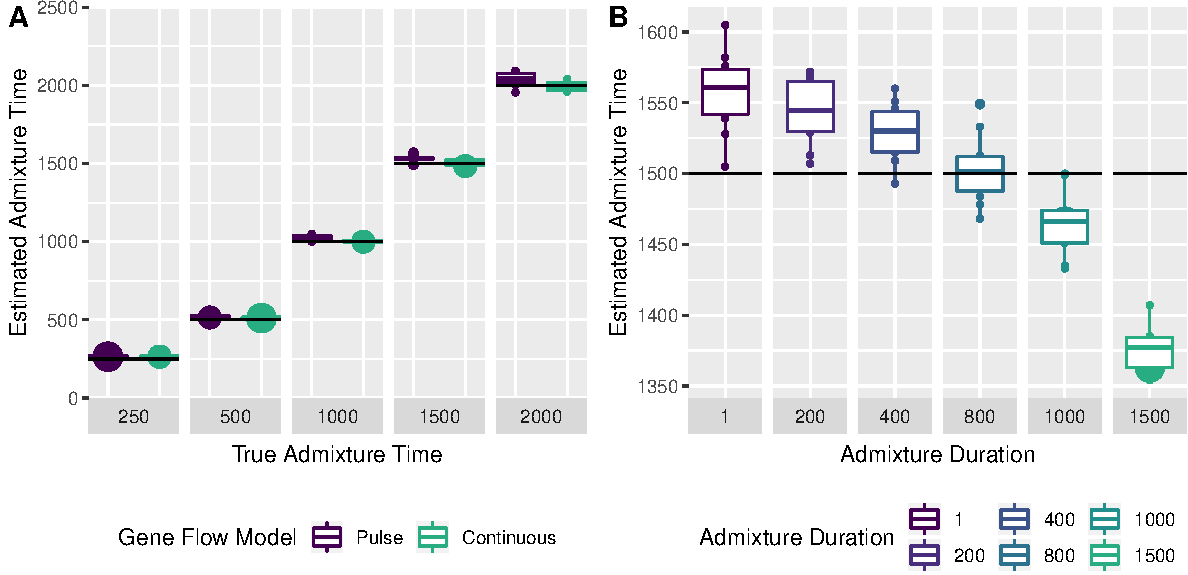
\includegraphics{Admixture_Time_Inference_Paper_Draft_files/figure-latex/fig2-1.pdf}
\caption{\label{fig:fig2} A) Comparison of mean admixture time estimates
between pulse and continuous gene flow for different admixture times.
The length of continuous gene flow corresponds to 50\% of the mean
admixture time, black line indicates true mean admixture time. B)
Comparison of mean admixture time estimates for simulations with a mean
time of admixture of 1500 generations ago, at a varying length of gene
flow. Boxplot created from 100 simulation replicates, respectively.}
\end{figure}
\subsection{Comparing effect sizes}\label{comparing effect sizes}

Having established that the duration of continuous admixture under ideal
circumstances is only marginally influential on admixture time
estimates, we want to compare its effect to more realistic simulation scenarios. Two common assumptions, namely knowing the recombination pattern and knowing the demographic history, were implicitly used in the previous simulations.
Previous studies reported that violations of these assumptions can have an effect on the admixture time estimates.
 Hence, we used the African-American genetic map and a more complex demography with substructure in the ancestral human population and additional gene flow between Africans and non-Africans after the Neadertal admixture ended (Figure \ref{fig:figS1}, for simulations under more realistic parameters. The genetic distance was assigned using the average recombination rate of the African-American genetic map.
 Furthermore, we altered the used scheme for ascertainment of SNPs for admixture informative sites. We compared the LES where only
positions in the admixed population are considered where both source
populations are diverged from each other, to an even stricter scheme. The Higher-Enrichment Scheme (HES) requiring additional
to the LES non-Africans to be polymorphic at a SNP. Additionally, we altered the minimal distance between pairs of SNPs for which the LD is calculated from 0.02 cM to 0.05 cM.



We simulated every combination of these parameter sets resulting in 32
different sets with 100 replications each (Supp. Fig. \ref{fig:figS2}).
A GLM was applied to estimate effect sizes of the four predictors being
ascertainment scheme, minimal distance, demography and recombination on
the bias of admixture estimates (Supplement Table \ref{tab:tableS1}).
Figure \ref{fig:fig3} shows the comparison of the standardized
difference between true and estimated time between the previously used
model (ascertainment = LES, \(d_{0} = 0.02 cM\), demography = simple and
recombination = constant) further refereed to as the standard model and
a model with one of the four parameter changed, respectively and the
corresponding model prediction. The previously observed overestimation
of the standard model was estimated to be 0.25 (0.22 - 0.29 95 \% CI)
standard deviation from the true admixture time. Every parameter change
results in lower estimates compared to the standard model, with the
biggest difference between a constant and a varying recombination (-1.76
- -1.7 95 \% CI) and the smallest differences between a pulse and
continuous gene flow model (-0.15 - -0.08 95 \% CI). Most accurate
estimates are achieved using the LES ascertainment scheme in combination
with a minimal distance of 0.05 cM. Additionally, the bias introduced by
the demography seems to depend on the used ascertainment scheme, since
only under the HES a difference between the simple and complex
demography is evident (Supp. Fig. \ref{fig:figS2}).

Overall the bias introduced by the ascertainment, minimal distance
cutoff, demography and admixture model are 10 \% or less of the true
mean admixture time. The major uncertainties in the admixture time
estimate arise from assuming a constant recombination rate. The
admixture time estimates for a pulse or a multi-generation admixture are similarly effected by the other modeling parameters.

\begin{figure}
\centering
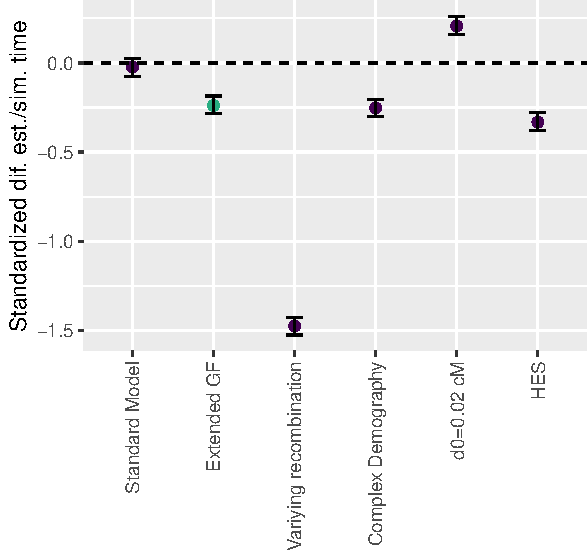
\includegraphics{Admixture_Time_Inference_Paper_Draft_files/figure-latex/fig3-1.pdf}
\caption{\label{fig:fig3} Comparison of the standardized difference between true and estimated admixture time for each parameter and the standard model of 100 replications each. Dotted line represents the model prediction with the 5.5 \% and 94.5 \% compatibility intervals solid lines. Dotted horizontal line indicates unbiased admixture estimates.}
\end{figure}

\subsection{Estimating the Lomax-parameters under different conditions}\label{estimating the Lomax-parameters under different conditions}

Building on the previous
result we wanted to find out the conditions to retrieve the Lomax
parameters i.e.~the duration of the admixture. We simulated an admixture
scenario under a simple demography with varying duration of continuous
admixture and sampled the population at different time points since the
end of the gene flow. Doing so allows us to examine how close one has to
sample form the end of a continuous admixture to still accurately
estimate its duration. Since the recombination map was shown to be highly
influential, we tested the duration estimates under a constant and variable
recombination using the HapMap genetic map. Here, we correct the
genetic distance by: assuming a constant rate, using the AAMap (uncertainty in the recombination map) or the
HapMap itself (knowing the population recombination map). We used the LES ascertainment scheme in combination with
a minimal distance of 0.05 cM. To fit the Lomax we can take advantage of
the fact that the bias of the mean time estimates using the simplified
one generation pulse model is relatively accurate. We can thus estimate
lambda first by fitting an exponential and in a second step estimating k
using a Lomax distribution with a starting parameter for lambda received
from the exponential fit, to archive better convergent. Figure \ref{fig:fig4} A and C show the mean
time estimates received from the Exponential fit. For simulations under a
constant recombination the mean time can be estimated confidently for different durations and different sampling times after the end of the admixture event. Estimates for simulation under a recombination map only
assuming a constant rate when calculating the LD results in severely
underestimation of the mean time estimates. Using the AAMap yields
results closer to the true value and less downwards biased, however only
using the exact same genetic map gives unbiased results. The mean time estimates received from the Lomax distribution show an overestimation on average and a higher variation (Supplement figure \ref{fig:figS2}).  Figure
\ref{fig:fig4} B and D shows the corresponding duration estimates by the
Lomax fit. Accurate estimates can be obtained throughout the different
gene flow length under a constant recombination rate, when sampled
recent from the end of the continuous admixture. Sampling further away from the end of the admixture results in less accurate estimates.  All simulations using a recombination map show a much higher
variance in the estimates. Especially for a gene flow length longer then
800 generations or sampled later then 50 generations away from the end
of the admixture, the estimates are not reliably. If no precise genetic map
is used to inferred the genetic distance between SNPs, no accurate
duration estimates can be obtained. The mean duration over all
replicates for the simulation corrected by the exact same map seems
relatively unbiased for a recent gene flow with a duration shorter 1000
generations. 

Under a realistic scenario with a varying recombination
rate, the duration can only be accurately estimated with a highly
precise map for recent continuous admixture events not longer then 400
generations. With regard to scenarios of Neandertal admixture,
accurately estimating the duration of possible continuous admixture from
present day human genomes even under a constant rate is
under powered. 
Figure \ref{fig:fig5} shows multiple gene flow duration scenarios ranging from a one generation pulse to 2500 generations of continuous gene flow. All scenarios are compatible with the ALD data from 1000 Genome's CEU computed using YRI and the Altai, Vindija and Chagyrskaya high coverage as reference populations and a CEU specific fine-scale genetic map.


Additionally, we tried to classifying the two admixture scenarios using  Akaike's information
criterion comparing the exponential model nested in the Lomax. We expect
that, since the AIC is penalizing extra parameter, that a Lomax fit to a
pulse like simulation scenario should be rejected, wheres for all the
other scenarios the Lomax would be preferred. However, for the
simplified simulation scenarios under a constant recombination rate were
we obtained the best results, the Lomax displays a lower AIC in 59 fits
out of 100 replications. Model comparison for scenarios of true
continuous admixture always resulted in the Lomax having a lower AIC.

\begin{figure}
\centering
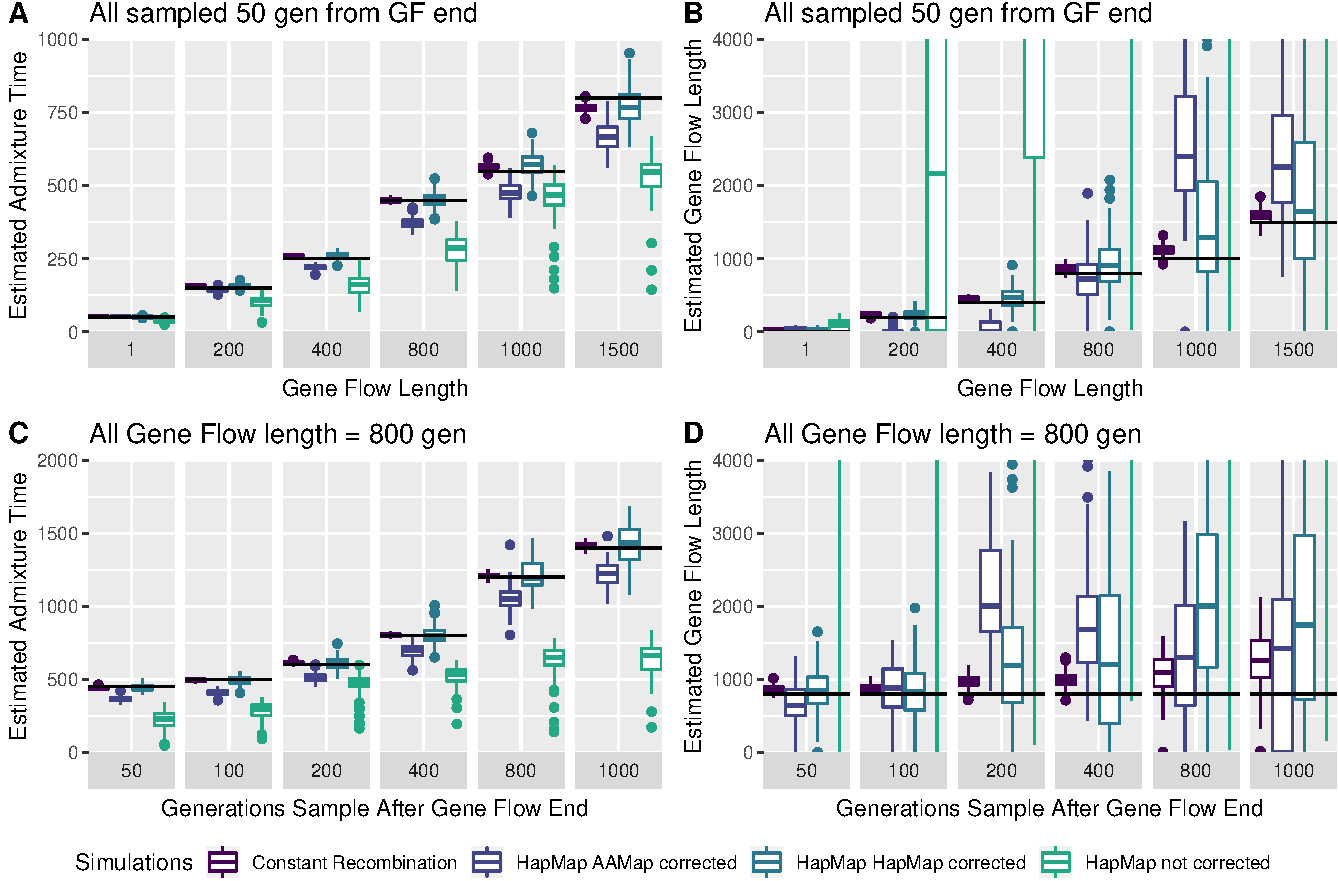
\includegraphics{Admixture_Time_Inference_Paper_Draft_files/figure-latex/fig4-1.pdf}
\caption{\label{fig:fig4} Parameter estimate for different sampling and
admixture duration times using different methods for assigning genetic
length A) Mean time estimates from the pulse model fit of different gene
flow length all sampled 50 generations after the gene flow ended. B)
Lomax duration estimate of the scenario C) Mean time estimates from the
pulse model fit of different sampling times after the end of 800
generations of gene flow. D) Lomax duration estimate of the scenario}
\end{figure}

\begin{figure}
\centering
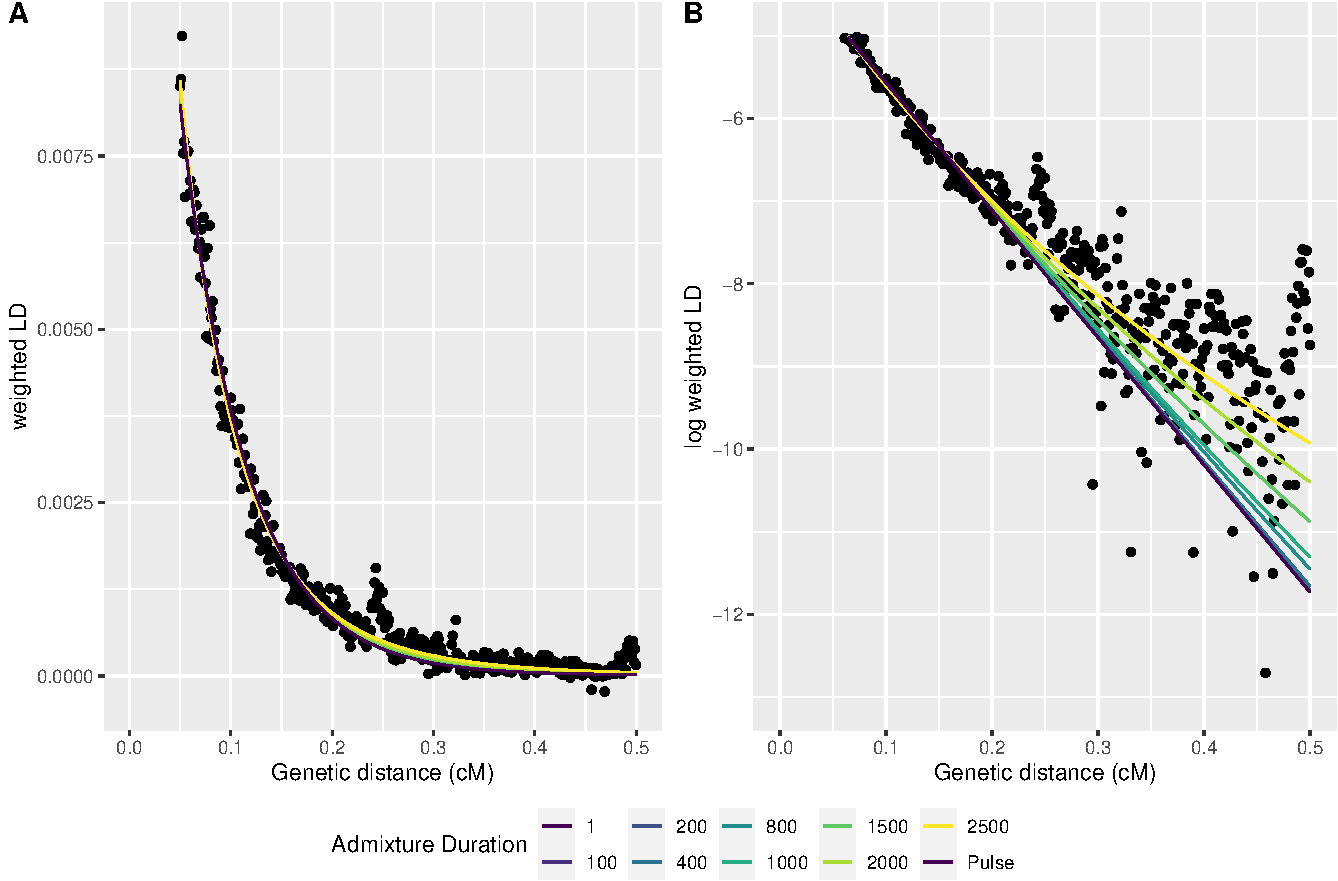
\includegraphics{Admixture_Time_Inference_Paper_Draft_files/figure-latex/fig5-1.pdf}
\caption{\label{fig:fig5} Different admixture duration models ranging
from a one generation pulse tu 2500 generations for Neandertal admixture
duration using all 1k Genome CEU individuals as the admixed population
with all YRI and 3 high coverage Neandertals as reference populations. A) Weighted LD normal scaled B) Weighted LD log scaled.}
\end{figure}

\section{Discussion}\label{discussion}

Archaeological evidence suggests that Neandertals and modern human populations overlapped in some regions for
a long period of time \citep{higham_timing_2014}, potentially resulting
in continuous admixture over hundreds of generations. However, estimates for the time of Neandertal-Human admixture usually assumes only a one-generation pulse. In this study we were interested in the effect of this assumption and to relax it. We established that even for very long continuous admixture scenarios, estimates for the mean time are compatible with a pulse like admixture and the error in the estimates is out weighted by all other tested model parameters.  Although, reliable estimates can be obtained, they in turn do not hold any information on the boundaries of a potential continuous admixture scenario. This however could be highly informative about the first contact between humans and Neandertals and the potential time of Neandertal extinction.

We tested the influence of different parameter scenarios on the admixture mean time estimates.
We established that assuming a constant recombination rate will lead to sever underestimations of admixture times, whereas the other parameters tested (demography and analysis parameters) are far less influential. Although this bias is known from previous studies, we notice it is underappreciated that reliable mean time estimates can only be obtained using population specific recombination maps, especially for archaic admixture events. Using the information on influencing parameters, we could obtain admixture durations modeling the ALD using a Lomax distribution under ideal circumstances, where we exactly know the genetic distance between introgressed SNPs and the recombination process is constant. Relaxation of the latter assumption while still knowing the exact population specific recombination map  leads to  uncertainty in the estimates. This uncertainty depend on the duration and time of sampling from the end of the admixture. Crucially we could show that there is no power to correctly infer admixture durations even for long admixture scenarios under ideal circumstances if the event is to long ago. Likewise, reliable distinction between a pulse like admixture model and a multi-generation continuous model for Human-Neandertal admixture scenarios is not definite. We demonstrated that a multitude of different duration scenarios are compatible for the Human-Neandertal admixture estimated from  present-day non-Africans genomes. Hence, we conclude that using present day non-African human genomes for inference is not conclusive to resolve the duration of Neandertal admixture. As a consequence we could neither obtain genetic indications of the first contact between Humans and Neandertals nor for the time of potential Neandertal extinction.

However, there are some ways to infer admixture event across time. Population differentiation between different introgressing archaic populations is a strong indicator for multi-generation admixture as shown in \cite{browning_analysis_2018}. Although not distinguishable by deconvoluting the length distribution of the archaic segments in the present-day East-Asian individuals to infer the time, the genetic differentiation between the segments with its implication of coming from different sources is unlikely to happen at the exact same time. Another possibility is using ancient DNA from admixed individuals to sample closer from the end of the admixture event. This could potentially help in either deconvolute discrete admixture pulses, which has the disadvantage of fitting multiple parameters or using our suggested approach on the ancient data. With a sufficient amount of ancient DNA samples from the same time period one could infer a recombination map. With that our study suggest that it would be possible to estimate a potential multi-generation admixture duration. One could also think of combining both ideas. Allocate introgressed segments from ancient DNA samples into different ancestry clusters according to their genetic differentiation and separately inferring mean and duration of the admixture time on each ancestry cluster. 

Conclusions:

\begin{itemize}
    \item The mean time of gene flow can be reliably estimated with a pulse model even if the gene flow is actually continuous. (check)
  \item Technical model variables (ascertainment scheme, minimal distance, demography and recombination map) outweigh the effect of continuous gene flow. (check)
  \item The Lomax model is under powered to inferring continuous admixture for parameters relevant for Neandertal admixture. (check)
  \item Estimating  the mean time and especially the duration of gene flow is only possible with a highly precise genetic map. (check)
  \item The signal of continuous gene flow is hard to detect if the gene flow is not long enough or to far in the past. (check)
  \item Reliably distinguishing the models is difficult. (check)
  \item Population differentiation can help identifying different admixture events across time (e.g. Browning et al. 2018)
  \item sampling close to the end of the admixture e.g. using ancient genomes and using a accurate recombination map enables the inference of admixture duration 
  
\end{itemize}

\hypertarget{refs}{}

\bibliography{References/MyLibraryATE}


\pagebreak
\setcounter{figure}{0} \renewcommand{\figurename}{Fig. S}
\renewcommand{\tablename}{Tab. S}

\section{Supplement}\label{supplement}

\begin{figure}
\centering
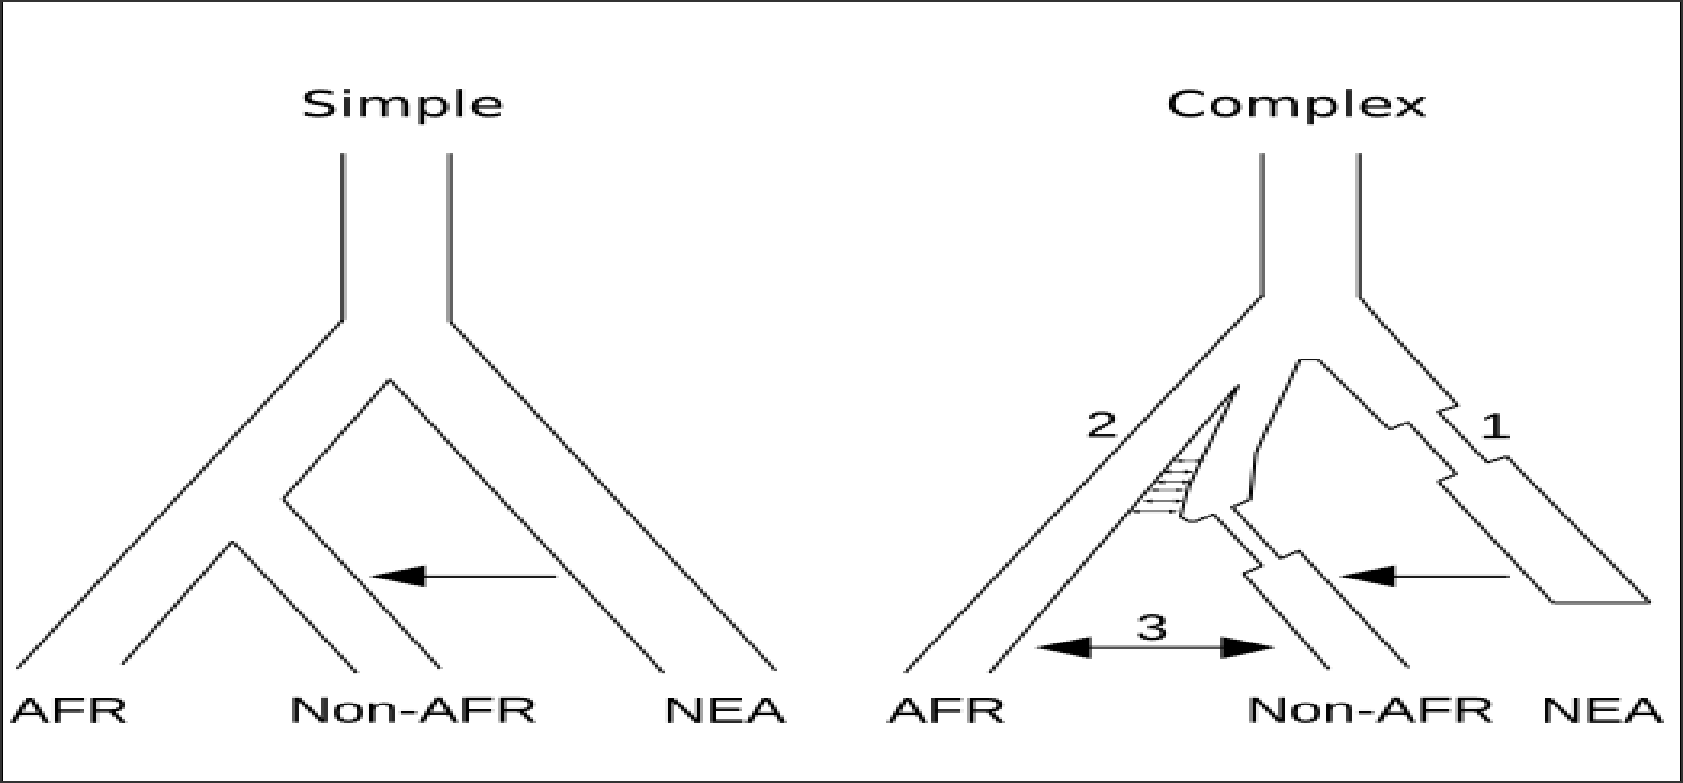
\includegraphics{Admixture_Time_Inference_Paper_Draft_files/figure-latex/figS1-1.pdf}
\caption{\label{fig:figS1}The two tested demographies of humans splitting into African population (AFR) and non-African (non-AFR) with admixture from Neandertals (NEA) into non-Africans. The simple demographic model with constant population sizes and the complex with rapid population size changes (1), substructure in Africa, where after an initial earlier split and isolation the structured population exchange migrants till the out-of-Africa event (2) and additional gene flow between Africans and non-Africans after the Neandertal admixture (3).}
\end{figure}

\begin{figure}
\centering
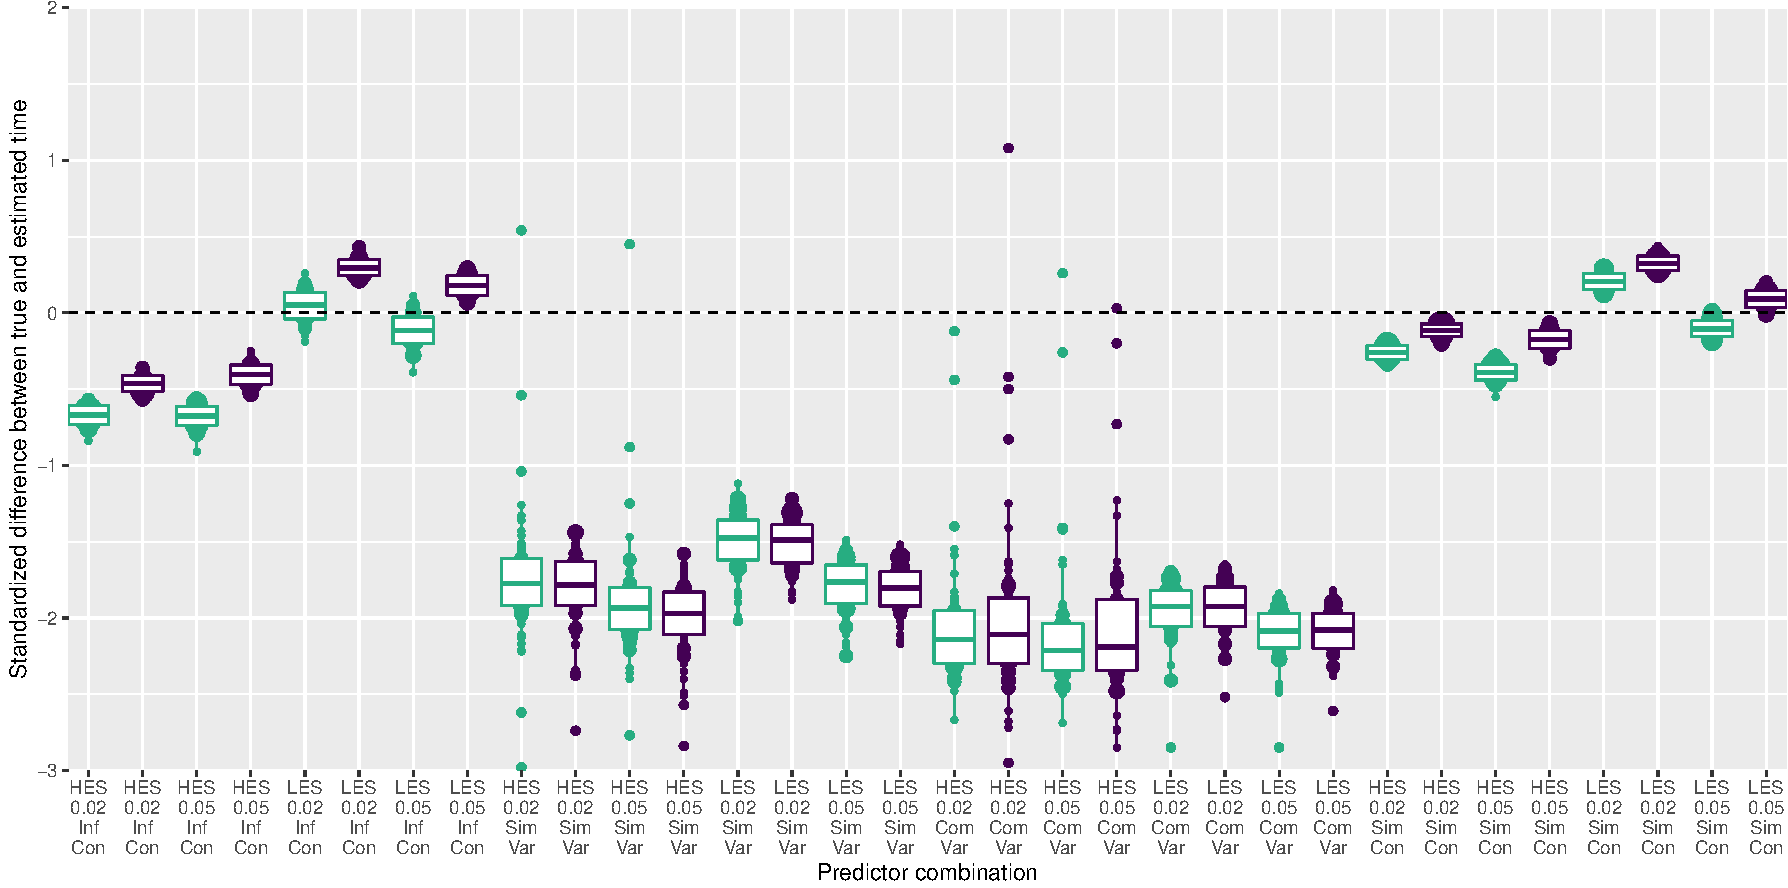
\includegraphics{Admixture_Time_Inference_Paper_Draft_files/figure-latex/figS2-1.pdf}
\caption{\label{fig:figS2} Comparison of the standardized difference between true and estimated admixture time for all combinations of parameters: ascertainment scheme = LES/HES,  $d_{0}$ = 0.02/0.05 cM, demography = simple/complex, recombination = constant/variable and the gene flow model = pulse/continuous, with 100 replicates respectively. Dotted line represents the model prediction with the 5.5 \% and 94.5 \% compatibility intervals solid lines. Dotted horizontal line indicates no difference between true and estimated time.}
\end{figure}

\begin{table}[h]
\caption{\label{tab:tableS1} Mean, standard deviation, 5.5/94.5 compatibility interval of the posterior distribution for every parameter effect on the standardized difference between true and estimated admixture time.}
\centering
\begin{tabular}{l|r|r|r|r|r|r}
\hline
  & mean & sd & 5.5\% & 94.5\% & n\_eff & Rhat\\
\hline
a & 0.25 & 0.02 & 0.22 & 0.29 & 1592.94 & 1\\
\hline
bG & -0.12 & 0.02 & -0.14 & -0.09 & 2053.35 & 1\\
\hline
bR & -1.73 & 0.02 & -1.76 & -1.70 & 2306.53 & 1\\
\hline
bD & -0.22 & 0.02 & -0.25 & -0.19 & 2281.65 & 1\\
\hline
bm & -0.13 & 0.02 & -0.16 & -0.11 & 2399.95 & 1\\
\hline
bA & -0.32 & 0.02 & -0.35 & -0.29 & 2250.29 & 1\\
\hline
sigma & 0.46 & 0.01 & 0.45 & 0.47 & 2538.23 & 1\\
\hline
\end{tabular}
\end{table}

\begin{figure}
\centering
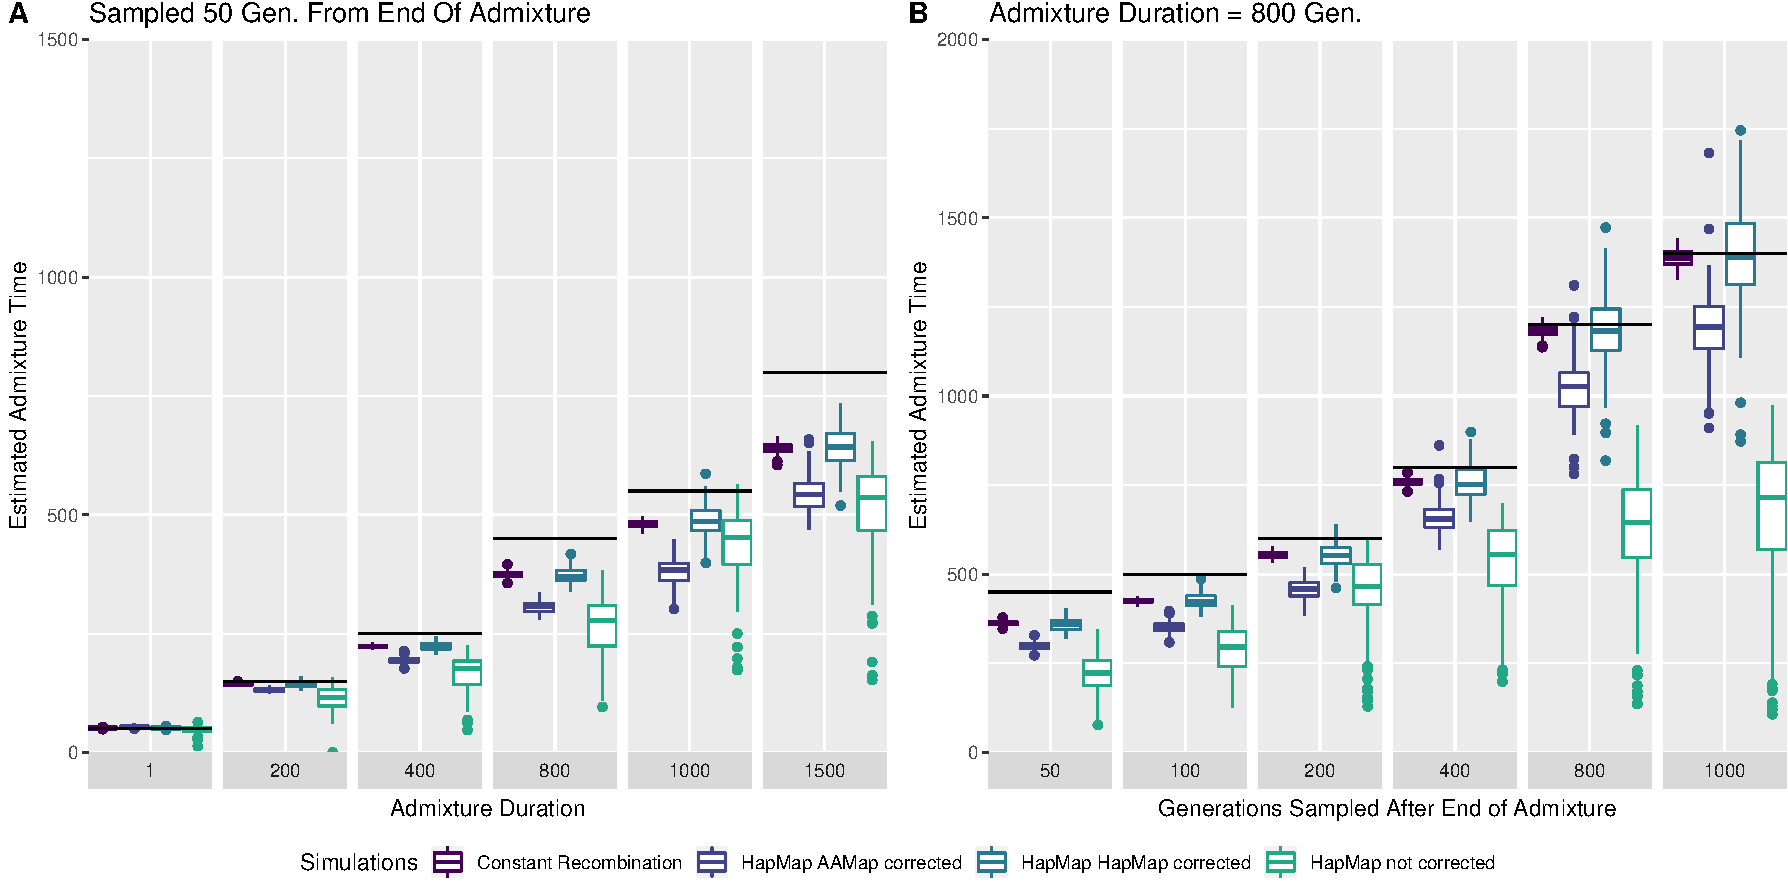
\includegraphics{Admixture_Time_Inference_Paper_Draft_files/figure-latex/figS3-1.pdf}
\caption{\label{fig:figS2} Comparison of mean time estimates between the Exponential and Lomax model A) Mean time estimates of the Exponential model fit for different 
admixture durations all sampled 50 generations after the admixture ended. B)
Lomax mean time estimate for the same scenario C) Mean time estimates of the Exponential model fit for different sampling times after the end of 800
generations of continuous admixture. D) Lomax mean time estimate for the same scenario}
\end{figure}


\end{document}